% Extension section (bonus). All numbers are macros from ../results/numbers_m4.tex.
\textbf{Question and hypotheses.} The paper motivates the cost~\eqref{eq:cost} by model quality but never
identifies a model. We test three hypotheses on the reproduced designs:
\textbf{E1} a model identified from the optimised input is more accurate over $\Dz$ than one identified
from a random-phase or Schroeder input with the same amplitude spectrum;
\textbf{E2} the gain survives when the design is computed on a model \emph{identified} from a first
random-phase experiment instead of the true system (the realistic case: the system to be identified is
unknown);
\textbf{E3} the space-filling cost is a useful predictor of model error.

\begin{figure}[t]\centering\footnotesize
\begin{tikzpicture}[node distance=3mm and 4mm,>=Stealth,
  b/.style={draw,rounded corners=2pt,align=center,inner sep=2.5pt,minimum height=7mm,fill=#1!10},b/.default=gray]
\node[b=blue] (r) {Exp.\,1: random\\phases $\varphi_0$};
\node[b=gray,right=of r] (id1) {identify\\$\hat g_1$ (ridge LS)};
\node[b=teal,right=of id1] (d1) {design on $\hat g_1$\\20 it.\ (adjoint)};
\node[b=teal,below=of d1] (e2) {Exp.\,2: \st{Osur}\\on true system};
\node[b=gray,left=of e2] (id2) {identify\\$\hat g_2$};
\node[b=black,left=of id2] (d2) {design on $\hat g_2$\\$\to$ \st{Oiter}};
\draw[->] (r)--(id1); \draw[->] (id1)--(d1); \draw[->] (d1)--(e2); \draw[->] (e2)--(id2); \draw[->] (id2)--(d2);
\end{tikzpicture}
\caption{Surrogate-in-the-loop design (E2): the true system is only used to run experiments; every design
step uses an identified model.}\label{fig:loop}\end{figure}

\textbf{Controlled design.} Only the phases differ between designs; spectrum (184 lines, std 160\,N),
length ($N=2048$, one steady-state period), model class, estimator and noise are identical.
Eight designs per seed $s=1\ldots20$: \st{R} random phases $\varphi_0(s)$; \st{S} Schroeder;
\st{O16}, \st{O20}, \st{Ofull}: the reproduced L-BFGS-B runs on the true system after 16, 20 and
$\le$1000 iterations; \st{Osur}: 20 iterations from $\varphi_0(s)$ on the model identified from the
\st{R} experiment, with the exact adjoint gradient propagated through the identified model;
\st{Oiter}: the model is re-identified from the \st{Osur} experiment and the design continued for 20
iterations (two-round sequential design, cf.\ \citealp{Pronzato2013}); \st{Osur100}: 100 iterations
on the first surrogate (40\,dB only).
\emph{Measurement}: both states are measured with white Gaussian sensor noise of \emph{fixed absolute}
level (a sensor does not know the input), set to 40 or 30\,dB below the state variance of the reference
random-phase signal, plus a noise-free case; the noise sequence of a seed is shared by all designs.
\emph{Model}: the kinematics $x_{1,k+1}=x_{1,k}+T_sx_{2,k}$ are known; the force law is a black box
$x_{2,k+1}=x_{2,k}+T_s\,\theta^\top\phi(z_k)$, with $\phi$ = constant, linear terms and 343 Gaussian
radial basis functions on a $7^3$ grid over $\Dz$ (width = spacing). RBFs are local, so they learn only
where data exist. \emph{Estimator}: ridge least squares on the one-step data,
$\hat\theta=(\Phi^\top\Phi+\lambda N I)^{-1}\Phi^\top y$, with $\lambda$ chosen by 5-fold blocked
cross-validation on the training data only \citep{Ljung1999}.
\emph{Tests} (never used for fitting or tuning): $e_{\mathrm{uni}}$, the NRMSE of $\hat g$ on 20\,000
points drawn uniformly in $\Dz$ (the region the user asked to model); $e_{\mathrm{sim}}$, the free-run
simulation NRMSE of $(x_1,x_2)$ on five new random-phase multisines at the design level (std 160\,N) and
at 1.5$\times$ that level (240\,N, stress test). \emph{Statistics}: medians over the 20 paired seeds and
a one-sided paired Wilcoxon signed-rank test against \st{R} \citep{Wilcoxon1945}, with a diverged simulation
ranked as the worst result. The $p$-values are unadjusted; all \mNTests{} tests are listed in the package,
and every $e_{\mathrm{uni}}$ improvement also survives a Bonferroni correction (all $p\le\mMaxPeuni$).
The two test types favour different designs: $e_{\mathrm{uni}}$ weights all of $\Dz$ equally, including
state combinations a random-phase input rarely reaches, while the random-phase free-run tests at 160\,N live
where random-phase training data are dense.

\begin{table}[t]\centering\scriptsize\setlength{\tabcolsep}{2.6pt}
\caption{Extension results, medians over \mNExt{} seeds. $^*$: better than random, $^\circ$: worse
than random (paired Wilcoxon, $p<0.01$); $^\dagger$: some free-run simulations diverged (counted as
failures). $C_\theta,\kappa$: coverage achieved on the true system.}
\label{tab:ext}% generated by m4_analysis.py
\begin{tabular}{@{}lrrrrrrr@{}}\toprule
 & \multicolumn{3}{c}{$e_{\mathrm{uni}}$ [\%]} & \multicolumn{2}{c}{$e_{\mathrm{sim}}$ [\%], 40 dB} & & \\
\cmidrule(lr){2-4}\cmidrule(lr){5-6}
Design & clean & 40\,dB & 30\,dB & 160\,N & 240\,N & $C_\theta$ & $\kappa$[\%]\\\midrule
random & 19.0 & 19.0 & 22.2 & 17.7 & 107.6$^\dagger$ & 251 & 37\\
Schroeder & 9.8$^{*}$ & 11.8$^{*}$ & 5.6$^{*}$ & 40.5$^{\circ}$ & 49.9$^{*}$ & 159 & 35\\
opt. 16 it. & 2.2$^{*}$ & 2.7$^{*}$ & 4.3$^{*}$ & 22.5 & 12.6$^{*}$ & 4.45 & 48\\
opt. 20 it. & 2.2$^{*}$ & 2.6$^{*}$ & 4.0$^{*}$ & 22.0 & 12.7$^{*}$ & 3.65 & 49\\
opt. full & 1.7$^{*}$ & 2.2$^{*}$ & 3.6$^{*}$ & 23.6 & 12.9$^{*}$ & 1.21 & 60\\
surrogate & 2.9$^{*}$ & 4.3$^{*}$ & 6.5$^{*}$ & 18.4 & 16.8$^\dagger$$^{*}$ & 46.6 & 45\\
iterative & 2.1$^{*}$ & 2.7$^{*}$ & 4.3$^{*}$ & 23.3$^{\circ}$ & 13.1$^{*}$ & 7.08 & 51\\
surr. 100 it. & -- & 3.7$^{*}$ & -- & 20.0 & 16.2$^\dagger$$^{*}$ & 42.7 & 47\\
\bottomrule\end{tabular}
\end{table}

\begin{figure*}[t]\centering
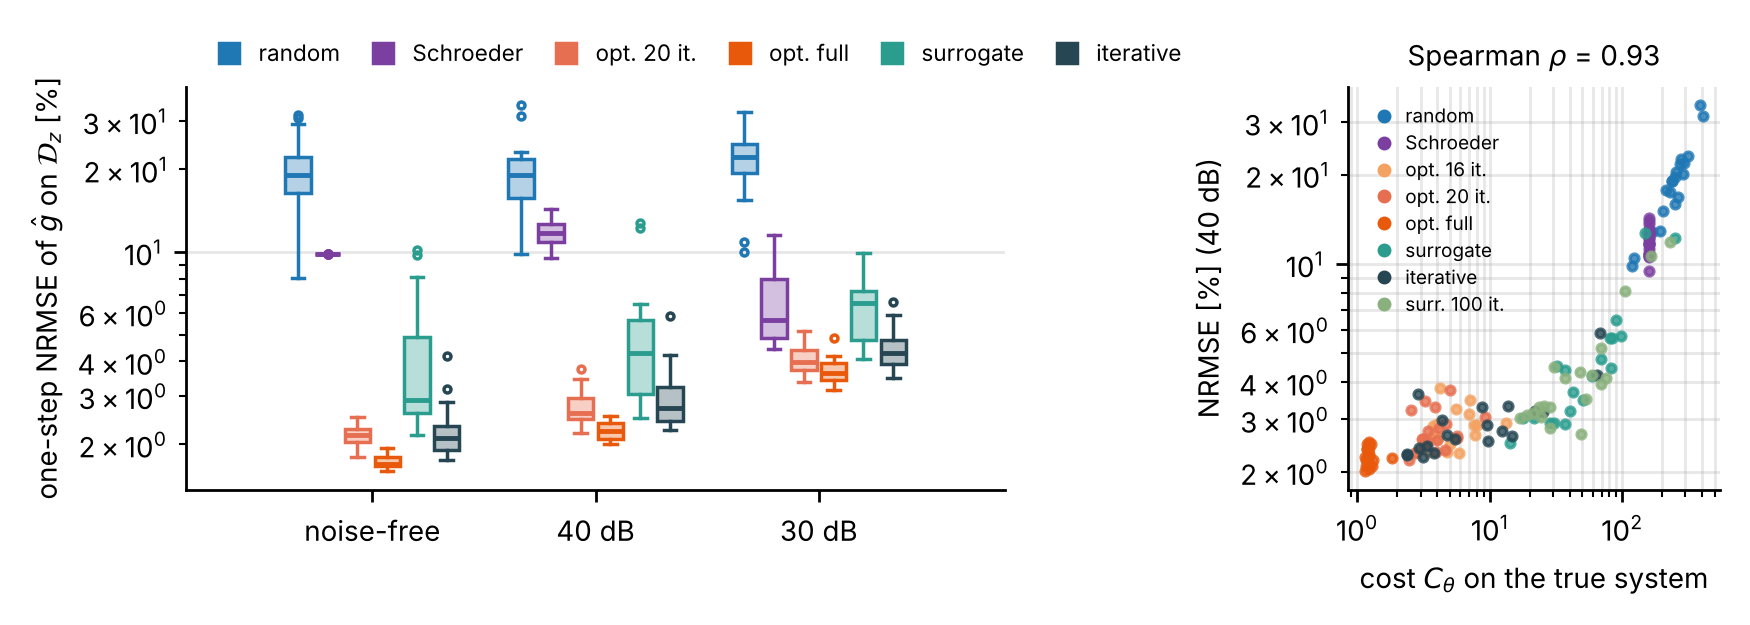
\includegraphics[width=0.85\textwidth]{fig_ext_accuracy.png}\\[2pt]
\small (a)\\[2pt]
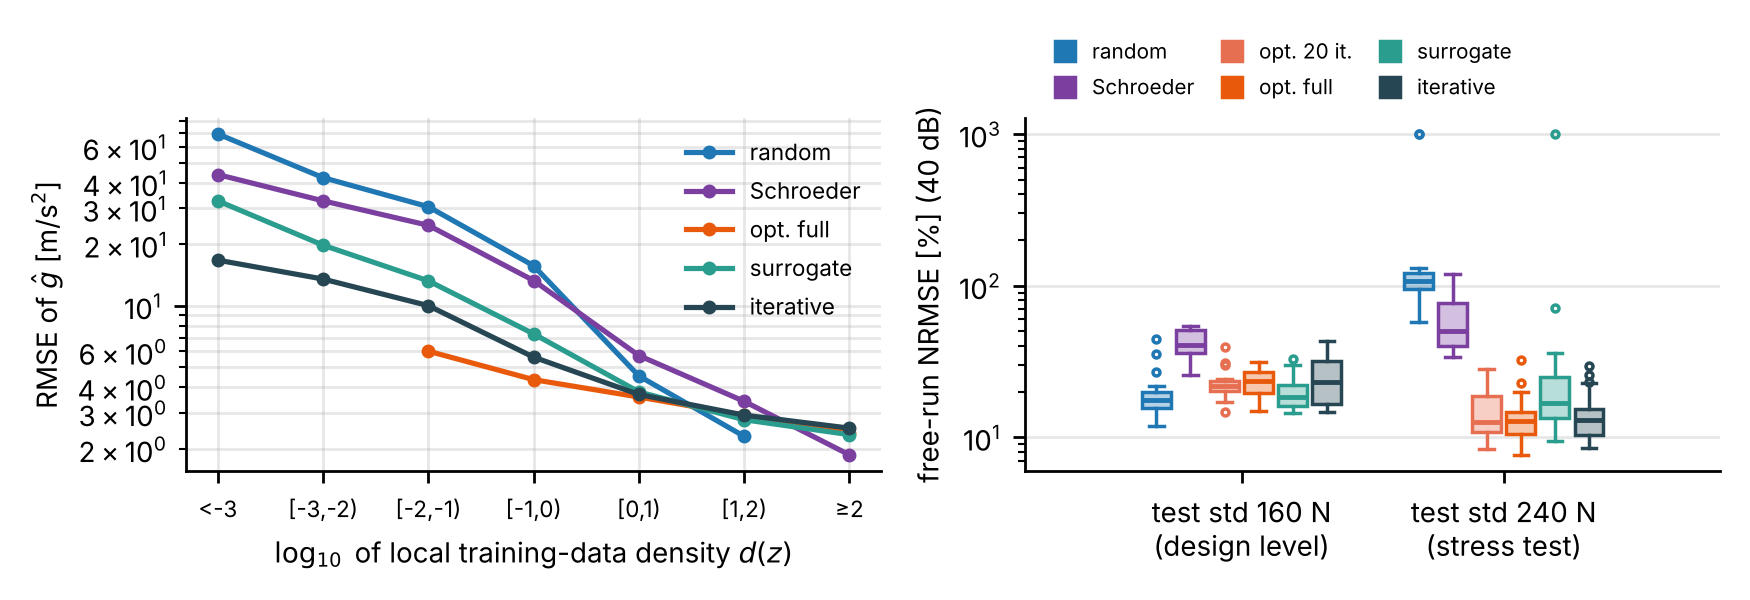
\includegraphics[width=0.85\textwidth]{fig_ext_mechanism.png}\\[2pt]
\small (b)
\caption{Extension, \mNExt{} seeds. (a) Left: one-step error of the identified force law over $\Dz$ for each
design and noise level. Right: model error vs.\ the space-filling cost achieved on the true system (40\,dB,
all designs and seeds). (b) Left: RMSE of $\hat g$ against the local density $d(z)$ of the training data
(40\,dB, pooled over seeds). Right: free-run simulation error on unseen random-phase multisines at the design
level (160\,N) and at 1.5$\times$ (240\,N); diverged runs are plotted at $10^3$\,\%.}
\label{fig:ext}\end{figure*}

\textbf{E1: coverage becomes accuracy.} Table~\ref{tab:ext} and Fig.~\ref{fig:ext}a: at 40\,dB the
median one-step error over $\Dz$ falls from \mXRfortyeuni\,\% (random) and \mXSfortyeuni\,\% (Schroeder)
to \mXOfullfortyeuni\,\% (optimised), a median paired improvement of \mFOfullforty$\times$
(\mWinOfullfortyeuni/\mNExt{} seeds better, $p$\,\mPOfullfortyeuni). The early-stopped designs, which
match the paper's cost level, already give \mFOtwentyforty$\times$, so most of the gain comes from the
first iterations. Schroeder also beats random phases over $\Dz$ (\mFSforty$\times$), but far less. The gain shrinks with noise (\mFOfullinf$\times$ clean, \mFOfullthirty$\times$ at
30\,dB) but stays significant. It is not an artefact of the cross-validated ridge parameter: with the same
fixed $\lambda$ for every design the gain is \mFixFAforty$\times$ ($\lambda=10^{-6}$) and
\mFixFBforty$\times$ ($\lambda=10^{-4}$) at 40\,dB. The Schroeder result, however, is sensitive to $\lambda$
(\mFixSAforty\,\% vs.\ \mFixSBforty\,\%), and its error even drops at 30\,dB, where cross-validation picks a
larger $\lambda$: for designs that leave parts of $\Dz$ empty, $e_{\mathrm{uni}}$ measures extrapolation, and
that depends on the regulariser. Fig.~\ref{fig:ext}b (left) shows the mechanism: for every design the error
falls with the local data density; the random-phase input leaves large parts of $\Dz$ at densities below
$10^{-2}$, where the model only extrapolates, while the optimised input leaves almost none.

\textbf{The price.} On free-run tests at the design level the picture changes: the random-phase test
signals live exactly where random-phase training data are dense, and there the random-phase model is as
good as or better than the optimised one (\mXRfortyesimonesixty\,\% vs.\
\mXOfullfortyesimonesixty\,\%; not significant at 1\,\%, $p$\mPwOfullfortyesimonesixty). The space-filling input spends the same number of samples on a larger
region, which is a bias--variance trade-off, not a free gain. At 1.5$\times$ the amplitude the
random-phase model fails (median \mXRfortyesimtwoforty\,\%, \mXRfortydivTot{} of its 200 free-run
simulations diverged) while the optimised one stays at \mXOfullfortyesimtwoforty\,\% with no divergence.
Schroeder, with the lowest crest factor, gives the worst free-run model at the design level
(\mXSfortyesimonesixty\,\%): it covers $x_1,x_2$ but not the input axis.

\textbf{E2: the design still works when the model is unknown.} Designing on a model identified from one
random-phase period keeps a \mFOsurforty$\times$ improvement (\mXOsurfortyeuni\,\%), even though the
surrogate predicts the coverage poorly: the true cost of \st{Osur} is \mXOsurfortyCtrue{} while the
surrogate predicted \mChatOsur; \mXOsurfortydivTot{} of its 200 free-run simulations diverged. One
re-identification round (\st{Oiter}) moves the true cost to \mXOiterfortyCtrue{} and the gain to
\mFOiterforty$\times$. Running 100 iterations on the first surrogate (\st{Osur100}) gives
\mFOsurOneZeroZeroforty$\times$ (true cost \mXOsurOneZeroZerofortyCtrue): the optimiser lowers the
\emph{surrogate's} cost, partly by exploiting its errors outside the data. The budgets differ: \st{Osur} and
\st{Osur100} use two experiments, \st{Oiter} three and 40 surrogate iterations; every final model is still
identified from one period of the last experiment only. In our runs, a second identification round gained
more than 80 extra iterations on the first surrogate; we did not test this difference statistically.

\textbf{E3: the cost predicts model quality, but only coarsely.} Across design families the space-filling
cost on the true system ranks the model error (pooled Spearman $\rho=\mRhoforty$ at 40\,dB, \mRhoinf{} clean,
\mRhothirty{} at 30\,dB; Fig.~\ref{fig:ext}a right; descriptive only, as the seeds of one design are not
independent families). It also holds within the random-phase designs ($\rho=\mRhoInR$) and over the
three optimised stopping points together ($\rho=\mRhoOpt$, $p$\mRhoOptP), but among the converged designs
alone it disappears ($\rho=\mRhoInOfull$, $p$\mRhoInPOfull): once $\Dz$ is well covered, further cost
reductions no longer predict the error. The cost is therefore a useful indicator of whether a dataset covers
$\Dz$, not a fine predictor of model accuracy; it also needs the measured or simulated states, so it can
only be checked after the experiment or on a model.
